%\subsection{Observations and motivation} % just find the proble and benefit
%\label{sec:background}
%
%\subsection{Need of Deduplication}
%
%In order to understand the extent of storage requirements and performance demands from a Docker registry. 
%We observe the amount of public repositories hosted by Docker Hub registries. 
%The number of public repositories is constantly increasing with a growth that amounts 
%to around one million repositories annually. 
%This corresponds to~130\,TB of annual growth in storage requirements (but it is acually less because of shared layers, right?), 
%costing around~\$15,000 a month if Google Cloud Storage is used~\cite{GoogleCloudStoragePricing}.
%This growth implies significant benefits to storage deduplication. 
%
%Deduplication option, block level, file level ...?
%
%
%
%\paragraph{Deduplication statistics} % the potiential of deduplication 
%
%how dedup will help
%
%
%layer ref count 
%
%\paragraph{Deduplication ratio growth} % benefit

\subsection{Need for User behavior based cache management}

%\paragraph{Access skewness}
%According to ~\cite{dockerworkload}, 
%\paragraph{Reuse time distribution}
%\subsubsection{Observations}

%\paragraph{Layers that belong to the same repo have different popularity}
\begin{figure}[t]
	\centering
		\begin{minipage}{0.225\textwidth}
			\centering
			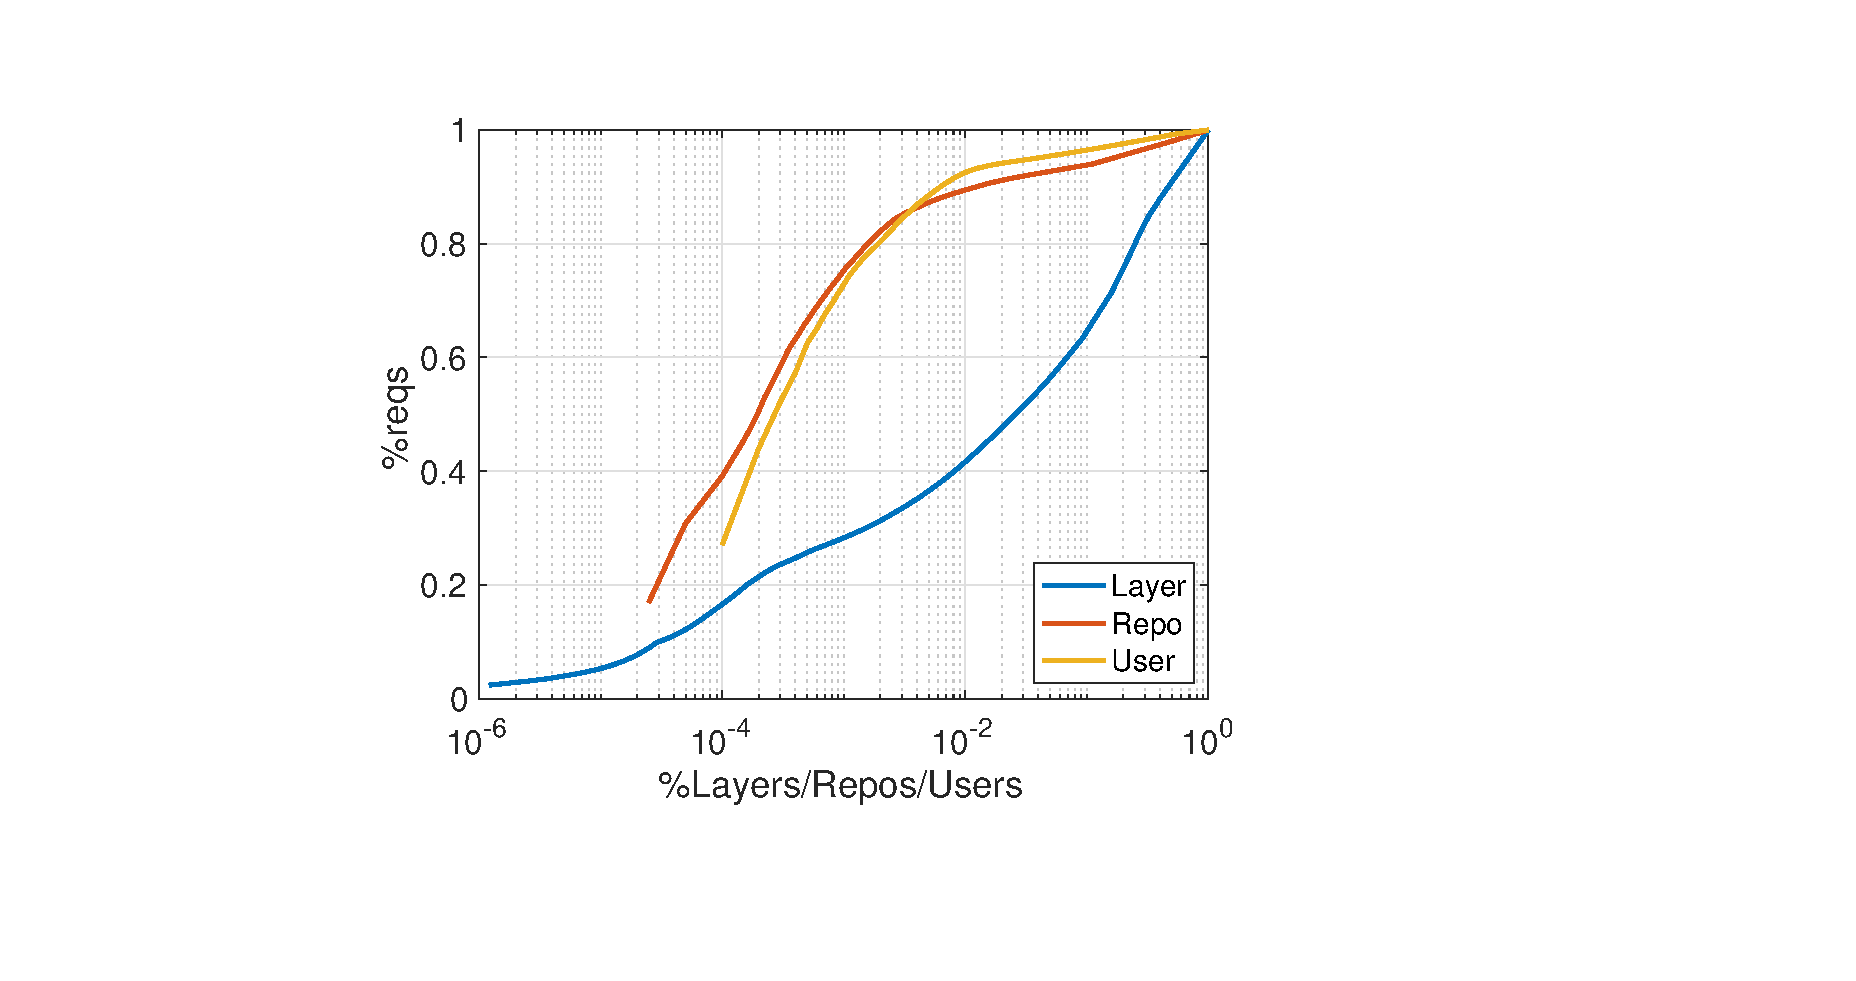
\includegraphics[width=1\textwidth]{graphs/skewness_cdf.eps}
			\caption{Popularity of layers, repos, and users.}
			\label{fig:sknewss}
		\end{minipage}
	\begin{minipage}{0.225\textwidth}
		\centering
		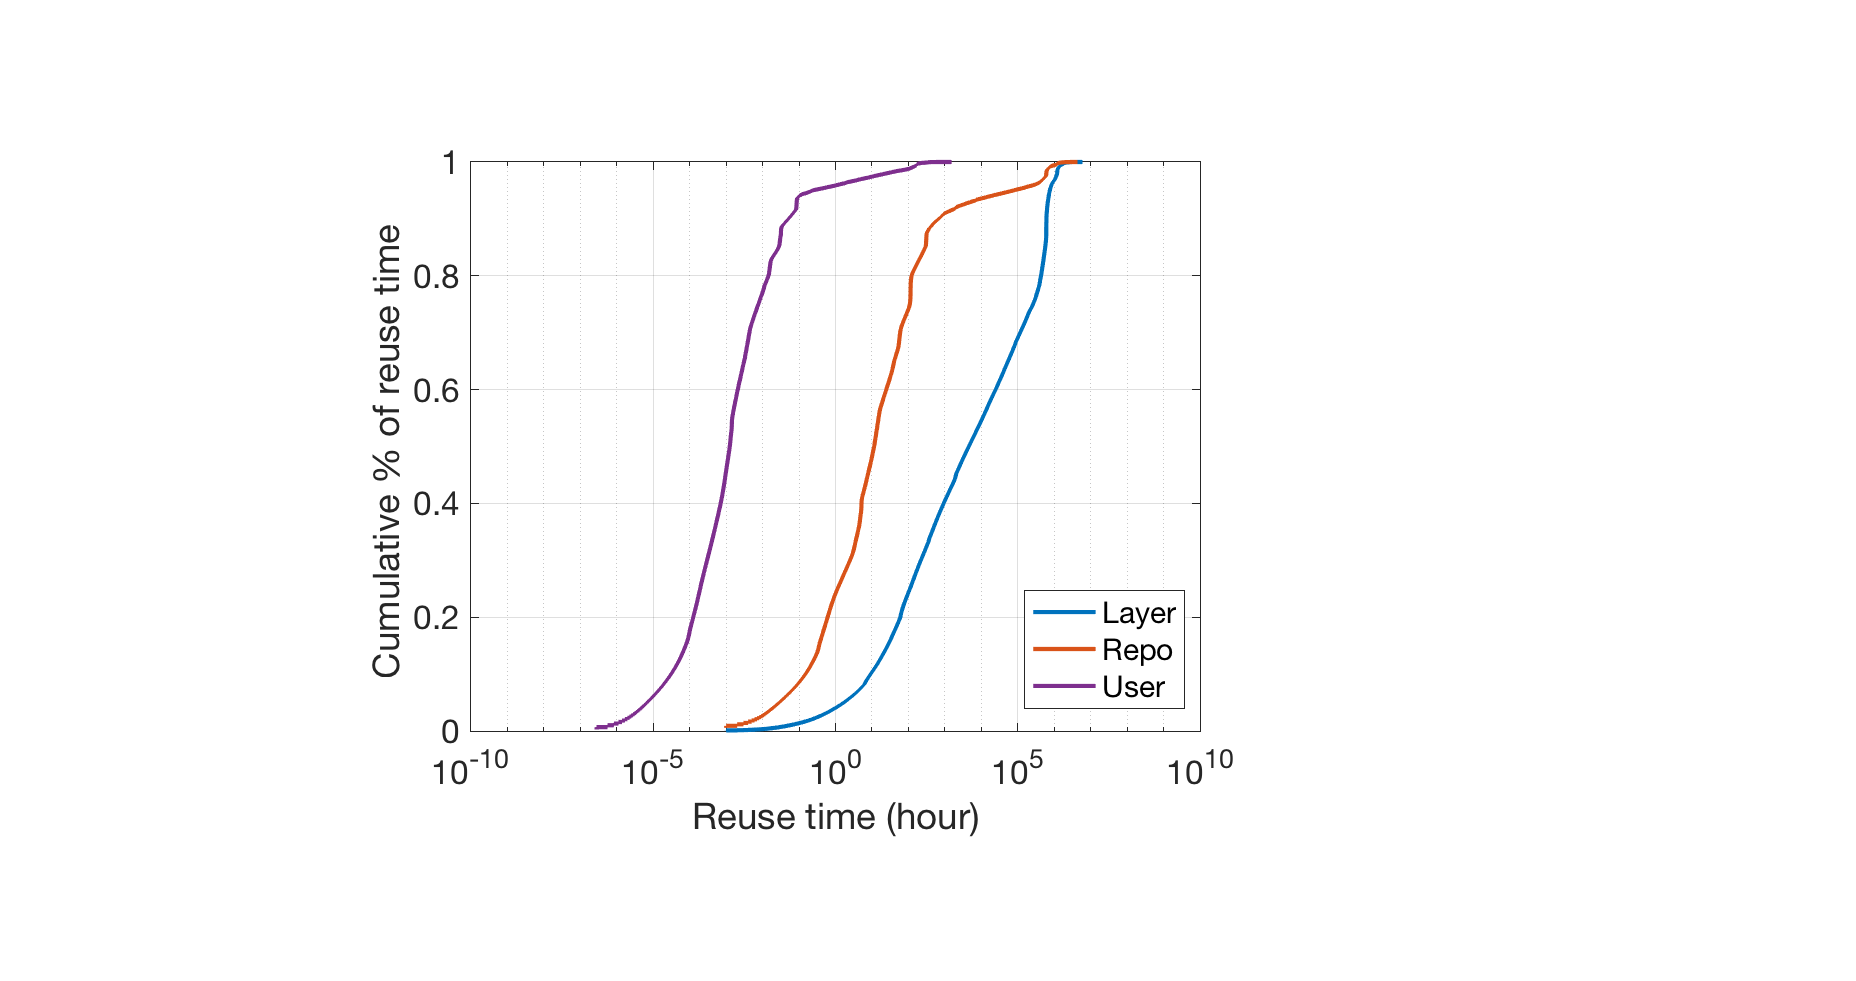
\includegraphics[width=1\textwidth]{graphs/reuse_time.eps}
		\caption{CDF of reuse time for layers, repos, and users.}
		\vspace{-3pt}
		\label{fig:reusetime}
	\end{minipage}
\end{figure}

\paragraph{Requests to layers are heavily skewed but layer reuse time is very long}
Figure~\ref{fig:sknewss} shows the registry accesses to layers, repositories, and by users for IBM container registry workload in Dallas(\texttt{dal})~\cite{dockerworkload}. There is heavy skew in layer access. For example, 25\% of popular layers account for 80\% of all requests. For repository accesses and accesses by users, skew is more significant than for layers. 10\% most frequently accessed repositories account for 94\% of all requests while 9\% most active users issued 97\% of all requests. Active users are the users that issue requests to registries.
This means few extremely active users create their repositories in \texttt{dal} and send majority of the requests.

Figure~\ref{fig:sknewss} shows the reuse time of layers, repositories, and by users. Reuse time is the duration between two subsequent requests that accesses the same layer or repository while reuse time by user is defined as duration between two subsequent requests that are issued by the same user. 
Layer reuse time is long.
The median reuse time for layer is 1.3 hour. While 80\% repositories experience the highest request frequency of reuse time around 2 minutes and 90\% users maintain active for at least 0.06 second.
So for a registry, most of its stored layers are not accessed frequently given a very short time period while
users can maintain active for a longer time. 
This is because users can access multiple layers and manifests.

\paragraph{User active time is predictable} 
Based on the above observations, we believe that user active time is predictable. 
By just maintaining a LRU list of users, we achieved 99\% accuracy for predicting user active time.
Therefore, we utilize the predictable user active time in our cache algorithm design.

